\chapter{Event reconstruction}

\intro{The reconstruction of basic analysis objects is described. A key ingredient in the \gls{cms} reconstruction is the particle flow algorithm which defines particle candidates by combining various subdetector information. The focus is set on the reconstruction of muons, electrons, jets and the missing transverse energy which are used in the study of single top quark production. }

The event reconstruction attempts to extract basic analysis objects from the raw detector data. In \gls{cms}, basic objects are particle tracks and vertices as well as charged lepton, photon, and jet candidates. During the reconstruction additional information such as the missing transverse energy, $\met$, and the likelihood of jets to originate from hadronization of b~quarks~(``b-tagging'') is determined. Since $\tau$ leptons and photons are not relevant for the study of $t$-channel single top quark production their reconstruction is omitted here.


%##############################################
\section{Track and vertex reconstruction}
%##############################################

The track reconstruction is split in two steps. First, in the local reconstruction, hits from charge distributions on the pixel and strip modules of the tracker are formed. Then, in the global reconstruction, trajectory candidate are seeded and build from compatible hits. A final fit to the found hits estimates the track parameters like the particle's momentum. The individual steps are described briefly in the following. More details can be found in Ref.~\cite{Chatrchyan:2014fea}.

Different algorithms are used to determine the local position of 2D (1D) hits from the distributions of charge deposits on the pixel (strips) respectively. For the pixels, a fast estimation of the hit position is performed for the track seeding and building stage. 

local pixel, strip hits, matched

seeding

trajectory building, pattern recognition, ghost

track fitting

quality, fakes, masking, iterative tracking

vertices, primary, secondary, 


\myfigure{\label{fig:reconstruction-trackingiter}The figure is taken from the public tracking result web page of CMS~\cite{trackingpublic}.}{
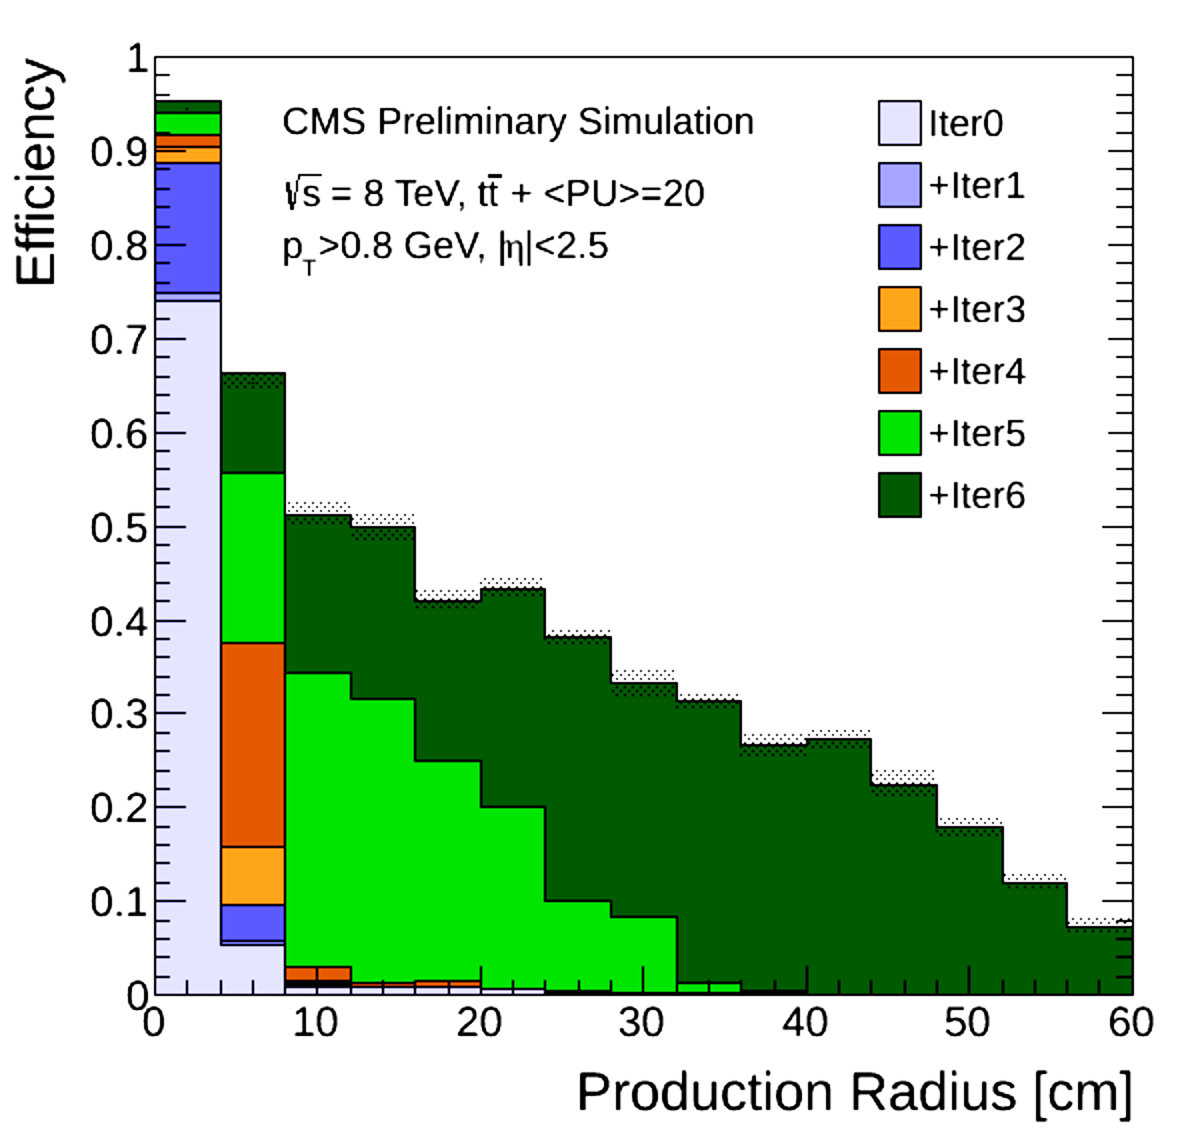
\includegraphics[width=0.45\textwidth]{figures/reconstruction/tracking_vs_vertpos.jpg}
}

%##############################################
\section{Particle flow}
%##############################################

%##############################################
\section{Muons}
%##############################################

%##############################################
\section{Electrons}
%##############################################

%##############################################
\section{Jets}
%##############################################

CHS, JEC, JER

%##############################################
\section{b-tagging}
%##############################################

SF, rizzi recipe

%##############################################
\section{Missing transverse energy}
%##############################################

T0, T1 corrections

%##############################################
\section{Luminosity and pileup}
%##############################################

pileup, rho
